\capitulo{3}{Conceptos teóricos}

La parte del proyecto más importante es el proceso de lanzar una aplicación Android desde cero, para ello se ha tenido que realizar una investigación para determinar que herramientas, lenguajes de programación, entornos de desarrollo son los más apropiados para un despliegue ágil.

Todo esto se sitúa en un mercado altamente competitivo, con una gran variabilidad (usuarios, empresas, desarrolladores ...) y con un constante cambio. 

\section{Framework}
Un framework (de origen anglosajón, marco de trabajo), según lo que dice la wikipedia~\cite{wiki:framework}, es una estructura conceptual y tecnológica de soporte definido, normalmente por módulos de software concretos, que sirve de base para la organización y el desarrollo de software. Las ventajas que ofrece son varias, entre las que se puede destacar:

\begin{itemize}
	\item \textbf{Evita repetición de código:} las partes más usadas, pasan a ser algo del \emph{core} del framework.
	\item \textbf{Uso de buenas prácticas:} muchos de estos están basados en patrones de diseño que nos obligan a usar.
	\item \textbf{Elementos avanzados integrados:} cosas complejas y que implementarlas llevaría mucho tiempo, suelen venir integradas.
	\item \textbf{Desarrollo ágil:} por los factores anteriores, podemos centrarnos más en la lógica de negocio de la aplicación que se desea hacer, de una manera más rápida y segura.
\end{itemize}

Por lo tanto, es necesario trabajar mediante frameworks, ya que nos garantizar una aplicación de mayor calidad, que si la hacemos desde cero, en código nativo.

\subsection{Opciones disponibles}
En el mercado existen muchos frameworks disponibles para el desarrollo de aplicaciones móviles, por lo que decantarse por uno no es tarea sencilla, ya que como se aprecia cada uno tiene sus pros y contras. En una encuesta realizada en un foro ~\cite{foro:encuesta}, a mediados del 2019, la opinión de los más recomendados era~\ref{fig:encuesta}:

\begin{figure}[h]
	\centering
	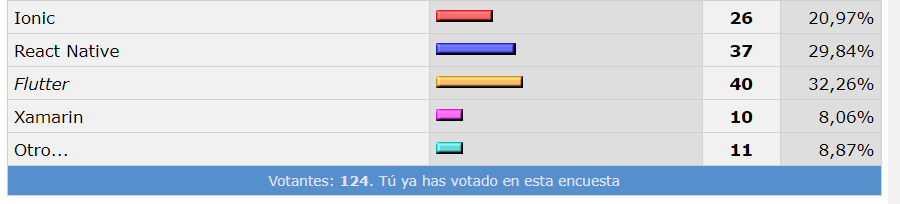
\includegraphics[width=1\textwidth]{teoria/encuesta.png}
	\caption{Encuesta}\label{fig:encuesta}
\end{figure}

Algo ideal es que se intento buscar un framework \emph{crossplataform}, con el que abarcar un mayor mercado, a nivel de usuarios y dispositivos.

\subsubsection{Ionic}
Ionic~\cite{wiki:ionnic} se basa en lenguaje de programación javascript, html y css. Internamente esta basado en otro framework, como es Angularjs. La licencia Open source, fue lanzado en el 2013, permite el desarrollo para iOS y Android. A sufrido gran cantidad de cambios desde entonces.

Ventajas:
\begin{itemize}
	\item Una amplia comunidad de usuarios.
	\item Documentación extensa y de calidad.
\end{itemize}

Algunas de las desventajas:
\begin{itemize}
	\item Rendimiento algo menor, ya que no se desarrolla de forma nativa.
	\item Bibliotecas en constante cambio y evolución, más que ser algo bueno, puede que deje a la aplicación fuera de versión y se tenga que hacer desde cero.
\end{itemize}

\subsubsection{React native}
React native~\cite{wiki:react} fue creado en 2015, de la mano de Facebook. La licencia que tiene es MIT. La diferencia que tiene con React, es que no manipula el DOM, por lo que tampoco usa HTML o CSS. 
Se programa en javascript. Las aplicaciones más conocidas que usan este framework es instgram o facebook.

Ventajas:
\begin{itemize}
	\item Gran comunidad de usuarios y herramientas.
	\item Mejora de las funcionalidades constantemente.
\end{itemize}

Algunas de las desventajas:
\begin{itemize}
	\item Rendimiento algo menor.
	\item No es código nativo, pero casi, por lo que no tiene soporte oficial de Google y Apple.
\end{itemize}

\subsubsection{Xamarin}
Xamarin~\cite{wiki:xamarin} creado por Microsoft en el 2011, por lo que está desarrollado en .NET, siendo propietario.

Ventajas:
\begin{itemize}
	\item Permite el desarrollo de iOS, Android, web pero nativas de escritorio también.
	\item Puede llamar a fragmentos de código usados en otras plataformas.
	\item Soporte para wearables.
\end{itemize}

Algunas de las desventajas:
\begin{itemize}
	\item Acceso limitado a las bibliotecas.
	\item Soporte y actualizaciones lento / tarde.
	\item Comunidad grande pero pequeña comparada con otras.
	\item Aplicaciones de mayor tamaño.
	\item Coste.
\end{itemize}

\subsubsection{Otros}
Hay muchos otros, cmomo kotlin, Apache Cordoba, jQuery Mobile, Native script ...
Pero no me convencieron por diversas razones. 
\section{Flutter}
